\documentclass[twoside]{book}

% Packages required by doxygen
\usepackage{fixltx2e}
\usepackage{calc}
\usepackage{doxygen}
\usepackage[export]{adjustbox} % also loads graphicx
\usepackage{graphicx}
\usepackage[utf8]{inputenc}
\usepackage{makeidx}
\usepackage{multicol}
\usepackage{multirow}
\PassOptionsToPackage{warn}{textcomp}
\usepackage{textcomp}
\usepackage[nointegrals]{wasysym}
\usepackage[table]{xcolor}

% Font selection
\usepackage[T1]{fontenc}
\usepackage[scaled=.90]{helvet}
\usepackage{courier}
\usepackage{amssymb}
\usepackage{sectsty}
\renewcommand{\familydefault}{\sfdefault}
\allsectionsfont{%
  \fontseries{bc}\selectfont%
  \color{darkgray}%
}
\renewcommand{\DoxyLabelFont}{%
  \fontseries{bc}\selectfont%
  \color{darkgray}%
}
\newcommand{\+}{\discretionary{\mbox{\scriptsize$\hookleftarrow$}}{}{}}

% Page & text layout
\usepackage{geometry}
\geometry{%
  a4paper,%
  top=2.5cm,%
  bottom=2.5cm,%
  left=2.5cm,%
  right=2.5cm%
}
\tolerance=750
\hfuzz=15pt
\hbadness=750
\setlength{\emergencystretch}{15pt}
\setlength{\parindent}{0cm}
\setlength{\parskip}{3ex plus 2ex minus 2ex}
\makeatletter
\renewcommand{\paragraph}{%
  \@startsection{paragraph}{4}{0ex}{-1.0ex}{1.0ex}{%
    \normalfont\normalsize\bfseries\SS@parafont%
  }%
}
\renewcommand{\subparagraph}{%
  \@startsection{subparagraph}{5}{0ex}{-1.0ex}{1.0ex}{%
    \normalfont\normalsize\bfseries\SS@subparafont%
  }%
}
\makeatother

% Headers & footers
\usepackage{fancyhdr}
\pagestyle{fancyplain}
\fancyhead[LE]{\fancyplain{}{\bfseries\thepage}}
\fancyhead[CE]{\fancyplain{}{}}
\fancyhead[RE]{\fancyplain{}{\bfseries\leftmark}}
\fancyhead[LO]{\fancyplain{}{\bfseries\rightmark}}
\fancyhead[CO]{\fancyplain{}{}}
\fancyhead[RO]{\fancyplain{}{\bfseries\thepage}}
\fancyfoot[LE]{\fancyplain{}{}}
\fancyfoot[CE]{\fancyplain{}{}}
\fancyfoot[RE]{\fancyplain{}{\bfseries\scriptsize Generated by Doxygen }}
\fancyfoot[LO]{\fancyplain{}{\bfseries\scriptsize Generated by Doxygen }}
\fancyfoot[CO]{\fancyplain{}{}}
\fancyfoot[RO]{\fancyplain{}{}}
\renewcommand{\footrulewidth}{0.4pt}
\renewcommand{\chaptermark}[1]{%
  \markboth{#1}{}%
}
\renewcommand{\sectionmark}[1]{%
  \markright{\thesection\ #1}%
}

% Indices & bibliography
\usepackage{natbib}
\usepackage[titles]{tocloft}
\setcounter{tocdepth}{3}
\setcounter{secnumdepth}{5}
\makeindex

% Hyperlinks (required, but should be loaded last)
\usepackage{ifpdf}
\ifpdf
  \usepackage[pdftex,pagebackref=true]{hyperref}
\else
  \usepackage[ps2pdf,pagebackref=true]{hyperref}
\fi
\hypersetup{%
  colorlinks=true,%
  linkcolor=blue,%
  citecolor=blue,%
  unicode%
}

% Custom commands
\newcommand{\clearemptydoublepage}{%
  \newpage{\pagestyle{empty}\cleardoublepage}%
}

\usepackage{caption}
\captionsetup{labelsep=space,justification=centering,font={bf},singlelinecheck=off,skip=4pt,position=top}

%===== C O N T E N T S =====

\begin{document}

% Titlepage & ToC
\hypersetup{pageanchor=false,
             bookmarksnumbered=true,
             pdfencoding=unicode
            }
\pagenumbering{alph}
\begin{titlepage}
\vspace*{7cm}
\begin{center}%
{\Large Decks and Dice }\\
\vspace*{1cm}
{\large Generated by Doxygen 1.8.13}\\
\end{center}
\end{titlepage}
\clearemptydoublepage
\pagenumbering{roman}
\tableofcontents
\clearemptydoublepage
\pagenumbering{arabic}
\hypersetup{pageanchor=true}

%--- Begin generated contents ---
\chapter{Hierarchical Index}
\section{Class Hierarchy}
This inheritance list is sorted roughly, but not completely, alphabetically\+:\begin{DoxyCompactList}
\item \contentsline{section}{card}{\pageref{classcard}}{}
\item \contentsline{section}{card\+Game}{\pageref{classcardGame}}{}
\begin{DoxyCompactList}
\item \contentsline{section}{War}{\pageref{classWar}}{}
\end{DoxyCompactList}
\item \contentsline{section}{card\+Game\+Factory}{\pageref{classcardGameFactory}}{}
\item \contentsline{section}{deck}{\pageref{classdeck}}{}
\item \contentsline{section}{dice}{\pageref{classdice}}{}
\item \contentsline{section}{dice\+Factory}{\pageref{classdiceFactory}}{}
\item \contentsline{section}{dice\+Game}{\pageref{classdiceGame}}{}
\begin{DoxyCompactList}
\item \contentsline{section}{pig}{\pageref{classpig}}{}
\end{DoxyCompactList}
\item \contentsline{section}{Leader\+Board}{\pageref{classLeaderBoard}}{}
\item \contentsline{section}{Menu}{\pageref{classMenu}}{}
\item \contentsline{section}{Player}{\pageref{classPlayer}}{}
\end{DoxyCompactList}

\chapter{Class Index}
\section{Class List}
Here are the classes, structs, unions and interfaces with brief descriptions\+:\begin{DoxyCompactList}
\item\contentsline{section}{\hyperlink{classcard}{card} \\*Card class represents a playing card with a suit and value }{\pageref{classcard}}{}
\item\contentsline{section}{\hyperlink{classcardGame}{card\+Game} \\*Card\+Game class creates a interface for all card games to follow }{\pageref{classcardGame}}{}
\item\contentsline{section}{\hyperlink{classcardGameFactory}{card\+Game\+Factory} \\*Card\+Game\+Factory class creates a factory that creates a card game }{\pageref{classcardGameFactory}}{}
\item\contentsline{section}{\hyperlink{classdeck}{deck} \\*Deck class creates deck of cards }{\pageref{classdeck}}{}
\item\contentsline{section}{\hyperlink{classdice}{dice} \\*Simulates the rolling of dice }{\pageref{classdice}}{}
\item\contentsline{section}{\hyperlink{classdiceFactory}{dice\+Factory} \\*Creates a faactory that produces dice games }{\pageref{classdiceFactory}}{}
\item\contentsline{section}{\hyperlink{classdiceGame}{dice\+Game} \\*Interface for all dice games to use }{\pageref{classdiceGame}}{}
\item\contentsline{section}{\hyperlink{classLeaderBoard}{Leader\+Board} \\*Provides Class representation of the \hyperlink{classLeaderBoard}{Leader\+Board} and ways to view the \hyperlink{classLeaderBoard}{Leader\+Board} }{\pageref{classLeaderBoard}}{}
\item\contentsline{section}{\hyperlink{classMenu}{Menu} \\*\hyperlink{classMenu}{Menu} Class represents the text based main menu which allows navigation of our program }{\pageref{classMenu}}{}
\item\contentsline{section}{\hyperlink{classpig}{pig} \\*Contains all the logic required for pig, a dice game }{\pageref{classpig}}{}
\item\contentsline{section}{\hyperlink{classPlayer}{Player} \\*Provides a class representation of everything a player has in and associated with a game }{\pageref{classPlayer}}{}
\item\contentsline{section}{\hyperlink{classWar}{War} \\*\hyperlink{classWar}{War} class contains all game logic for the card game war }{\pageref{classWar}}{}
\end{DoxyCompactList}

\chapter{Class Documentation}
\hypertarget{classcard}{}\section{card Class Reference}
\label{classcard}\index{card@{card}}


Card class represents a playing card with a suit and value.  




{\ttfamily \#include $<$Card.\+h$>$}

\subsection*{Public Member Functions}
\begin{DoxyCompactItemize}
\item 
\hyperlink{classcard_acfb86f1ab0161ad4445c6d08c2aa5bb5}{card} (int suit, int value)
\begin{DoxyCompactList}\small\item\em Card constructor creates a Card object. \end{DoxyCompactList}\item 
int \hyperlink{classcard_a952559b02cf7d0c468fb4d89e145ad48}{get\+Suit} ()
\begin{DoxyCompactList}\small\item\em get\+Suit gets the suit value as an integer \end{DoxyCompactList}\item 
int \hyperlink{classcard_a5cf12898a17ff2eda5469eaf857e286d}{get\+Value} ()
\begin{DoxyCompactList}\small\item\em get\+Value gets the card value as an integer \end{DoxyCompactList}\item 
std\+::string \hyperlink{classcard_a1038b6c4a093a84ccdea7e3b191dcadd}{get\+Suit\+Name} ()
\begin{DoxyCompactList}\small\item\em get\+Suit gets the suit value as an String \end{DoxyCompactList}\item 
std\+::string \hyperlink{classcard_a1fb74af5bd396a5b721adedf3f04af17}{get\+Value\+Name} ()
\begin{DoxyCompactList}\small\item\em get\+Value gets the card value as an String \end{DoxyCompactList}\end{DoxyCompactItemize}
\subsection*{Private Attributes}
\begin{DoxyCompactItemize}
\item 
\mbox{\Hypertarget{classcard_aa10e2884f273f75aa313a8bb5a6251f3}\label{classcard_aa10e2884f273f75aa313a8bb5a6251f3}} 
const int {\bfseries A\+CE} = 1
\item 
\mbox{\Hypertarget{classcard_a6b40b986e5bf417dc80ac4b6ef90d1a1}\label{classcard_a6b40b986e5bf417dc80ac4b6ef90d1a1}} 
const int {\bfseries J\+A\+CK} = 11
\item 
\mbox{\Hypertarget{classcard_aa09c255786e6ee4d89f731aa500fd07a}\label{classcard_aa09c255786e6ee4d89f731aa500fd07a}} 
const int {\bfseries Q\+U\+E\+EN} = 12
\item 
\mbox{\Hypertarget{classcard_a3dc8786d461be27ba29989676cdd4e44}\label{classcard_a3dc8786d461be27ba29989676cdd4e44}} 
const int {\bfseries K\+I\+NG} = 13
\item 
\mbox{\Hypertarget{classcard_acfc456145e637a32f29657fb25964f30}\label{classcard_acfc456145e637a32f29657fb25964f30}} 
const int {\bfseries S\+P\+A\+DE} = 1
\item 
\mbox{\Hypertarget{classcard_ac2613bacd68296da2362a74fd3972c8c}\label{classcard_ac2613bacd68296da2362a74fd3972c8c}} 
const int {\bfseries C\+L\+UB} = 2
\item 
\mbox{\Hypertarget{classcard_ad702ec3223c4b79a958a6ebd56887a32}\label{classcard_ad702ec3223c4b79a958a6ebd56887a32}} 
const int {\bfseries H\+E\+A\+RT} = 3
\item 
\mbox{\Hypertarget{classcard_a7a30e10aeb7f2f1d6c766dd37aa8ac16}\label{classcard_a7a30e10aeb7f2f1d6c766dd37aa8ac16}} 
const int {\bfseries D\+I\+A\+M\+O\+ND} = 4
\item 
\mbox{\Hypertarget{classcard_a173236802fa7d0c52e411523ae9d30fa}\label{classcard_a173236802fa7d0c52e411523ae9d30fa}} 
int {\bfseries suit}
\item 
\mbox{\Hypertarget{classcard_a8c8ecc859e715ee6b55bef5d692f508b}\label{classcard_a8c8ecc859e715ee6b55bef5d692f508b}} 
int {\bfseries value}
\end{DoxyCompactItemize}


\subsection{Detailed Description}
Card class represents a playing card with a suit and value. 

Card class provides functions to convert number values of cards to their string representation. ~\newline
Face values are\+: 1 being Ace, 11 being Jack, 12 being Queen, 13 being King ~\newline
Suit values are\+: 1 being Spade, 2 being Club, 3 being Heart, 4 being Diamond \begin{DoxyAuthor}{Author}
Jacob Ross 250892852 
\end{DoxyAuthor}


\subsection{Constructor \& Destructor Documentation}
\mbox{\Hypertarget{classcard_acfb86f1ab0161ad4445c6d08c2aa5bb5}\label{classcard_acfb86f1ab0161ad4445c6d08c2aa5bb5}} 
\index{card@{card}!card@{card}}
\index{card@{card}!card@{card}}
\subsubsection{\texorpdfstring{card()}{card()}}
{\footnotesize\ttfamily card\+::card (\begin{DoxyParamCaption}\item[{int}]{suit,  }\item[{int}]{value }\end{DoxyParamCaption})}



Card constructor creates a Card object. 

Card constructor creates a Card object using numbers to represent the values of the cards. 
\begin{DoxyParams}{Parameters}
{\em value} & Face values are\+: 1 being Ace, 11 being Jack, 12 being Queen, 13 being King \\
\hline
{\em suit} & Suit values are\+: 1 being Spade, 2 being Club, 3 being Heart, 4 being Diamond \\
\hline
\end{DoxyParams}
\begin{DoxyReturn}{Returns}
card object 
\end{DoxyReturn}
\begin{DoxyAuthor}{Author}
Jacob Ross 250892852 
\end{DoxyAuthor}


\subsection{Member Function Documentation}
\mbox{\Hypertarget{classcard_a952559b02cf7d0c468fb4d89e145ad48}\label{classcard_a952559b02cf7d0c468fb4d89e145ad48}} 
\index{card@{card}!get\+Suit@{get\+Suit}}
\index{get\+Suit@{get\+Suit}!card@{card}}
\subsubsection{\texorpdfstring{get\+Suit()}{getSuit()}}
{\footnotesize\ttfamily int card\+::get\+Suit (\begin{DoxyParamCaption}{ }\end{DoxyParamCaption})}



get\+Suit gets the suit value as an integer 

Face values are\+: 1 being Ace, 11 being Jack, 12 being Queen, 13 being King \begin{DoxyReturn}{Returns}
suit value as an integer 
\end{DoxyReturn}
\begin{DoxyAuthor}{Author}
Jacob Ross 250892852 
\end{DoxyAuthor}
\mbox{\Hypertarget{classcard_a1038b6c4a093a84ccdea7e3b191dcadd}\label{classcard_a1038b6c4a093a84ccdea7e3b191dcadd}} 
\index{card@{card}!get\+Suit\+Name@{get\+Suit\+Name}}
\index{get\+Suit\+Name@{get\+Suit\+Name}!card@{card}}
\subsubsection{\texorpdfstring{get\+Suit\+Name()}{getSuitName()}}
{\footnotesize\ttfamily string card\+::get\+Suit\+Name (\begin{DoxyParamCaption}{ }\end{DoxyParamCaption})}



get\+Suit gets the suit value as an String 

Suit values are\+: 1 being Spade, 2 being Club, 3 being Heart, 4 being Diamond \begin{DoxyReturn}{Returns}
suit value as an String 
\end{DoxyReturn}
\begin{DoxyAuthor}{Author}
Jacob Ross 250892852 
\end{DoxyAuthor}
\mbox{\Hypertarget{classcard_a5cf12898a17ff2eda5469eaf857e286d}\label{classcard_a5cf12898a17ff2eda5469eaf857e286d}} 
\index{card@{card}!get\+Value@{get\+Value}}
\index{get\+Value@{get\+Value}!card@{card}}
\subsubsection{\texorpdfstring{get\+Value()}{getValue()}}
{\footnotesize\ttfamily int card\+::get\+Value (\begin{DoxyParamCaption}{ }\end{DoxyParamCaption})}



get\+Value gets the card value as an integer 

Suit values are\+: 1 being Spade, 2 being Club, 3 being Heart, 4 being Diamond \begin{DoxyReturn}{Returns}
card value as an integer 
\end{DoxyReturn}
\begin{DoxyAuthor}{Author}
Jacob Ross 250892852 
\end{DoxyAuthor}
\mbox{\Hypertarget{classcard_a1fb74af5bd396a5b721adedf3f04af17}\label{classcard_a1fb74af5bd396a5b721adedf3f04af17}} 
\index{card@{card}!get\+Value\+Name@{get\+Value\+Name}}
\index{get\+Value\+Name@{get\+Value\+Name}!card@{card}}
\subsubsection{\texorpdfstring{get\+Value\+Name()}{getValueName()}}
{\footnotesize\ttfamily string card\+::get\+Value\+Name (\begin{DoxyParamCaption}{ }\end{DoxyParamCaption})}



get\+Value gets the card value as an String 

Face values are\+: 1 being Ace, 11 being Jack, 12 being Queen, 13 being King \begin{DoxyReturn}{Returns}
card value as an String 
\end{DoxyReturn}
\begin{DoxyAuthor}{Author}
Jacob Ross 250892852 
\end{DoxyAuthor}


The documentation for this class was generated from the following files\+:\begin{DoxyCompactItemize}
\item 
Base\+Card/Card.\+h\item 
Base\+Card/Card.\+cpp\end{DoxyCompactItemize}

\hypertarget{classcardGame}{}\section{card\+Game Class Reference}
\label{classcardGame}\index{card\+Game@{card\+Game}}


Card\+Game class creates a interface for all card games to follow.  




{\ttfamily \#include $<$card\+Game.\+h$>$}



Inheritance diagram for card\+Game\+:\nopagebreak
\begin{figure}[H]
\begin{center}
\leavevmode
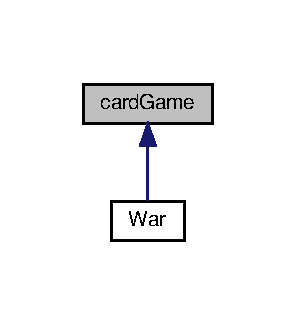
\includegraphics[width=142pt]{classcardGame__inherit__graph}
\end{center}
\end{figure}


Collaboration diagram for card\+Game\+:\nopagebreak
\begin{figure}[H]
\begin{center}
\leavevmode
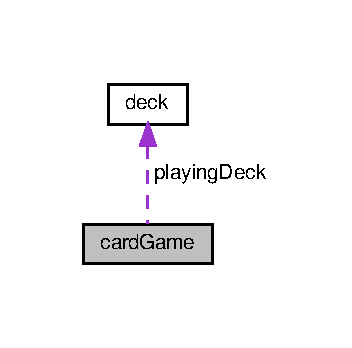
\includegraphics[width=169pt]{classcardGame__coll__graph}
\end{center}
\end{figure}
\subsection*{Public Member Functions}
\begin{DoxyCompactItemize}
\item 
\hyperlink{classcardGame_a9f128c2ea5d426a79b506ed02771bdbc}{card\+Game} ()
\begin{DoxyCompactList}\small\item\em Card\+Game constructor creates a base card game. \end{DoxyCompactList}\item 
\hyperlink{classcardGame_a23e7135b422d487d761b475713cf2e7a}{$\sim$card\+Game} ()
\begin{DoxyCompactList}\small\item\em Card\+Game deconstructor frees memory for objects being used. \end{DoxyCompactList}\item 
virtual void \hyperlink{classcardGame_ae8e04249f37f61e3adfa03cfbad3b021}{play} ()=0
\begin{DoxyCompactList}\small\item\em play function contains all game logic, run to play \end{DoxyCompactList}\end{DoxyCompactItemize}
\subsection*{Private Attributes}
\begin{DoxyCompactItemize}
\item 
\mbox{\Hypertarget{classcardGame_aa0db8fdd6a95e1dda328150c5bc6ed94}\label{classcardGame_aa0db8fdd6a95e1dda328150c5bc6ed94}} 
\hyperlink{classdeck}{deck} $\ast$ {\bfseries playing\+Deck}
\item 
\mbox{\Hypertarget{classcardGame_ad90e58da175c9cb069c8617d9455562d}\label{classcardGame_ad90e58da175c9cb069c8617d9455562d}} 
std\+::vector$<$ \hyperlink{classPlayer}{Player} $\ast$ $>$ {\bfseries player\+List}
\end{DoxyCompactItemize}


\subsection{Detailed Description}
Card\+Game class creates a interface for all card games to follow. 

Card\+Game class provides all card games a deck of cards and a player list to let the programmer use in game logic. \begin{DoxyAuthor}{Author}
Jacob Ross 250892852 
\end{DoxyAuthor}


\subsection{Constructor \& Destructor Documentation}
\mbox{\Hypertarget{classcardGame_a9f128c2ea5d426a79b506ed02771bdbc}\label{classcardGame_a9f128c2ea5d426a79b506ed02771bdbc}} 
\index{card\+Game@{card\+Game}!card\+Game@{card\+Game}}
\index{card\+Game@{card\+Game}!card\+Game@{card\+Game}}
\subsubsection{\texorpdfstring{card\+Game()}{cardGame()}}
{\footnotesize\ttfamily card\+Game\+::card\+Game (\begin{DoxyParamCaption}{ }\end{DoxyParamCaption})}



Card\+Game constructor creates a base card game. 

Card\+Game constructor creates a base card game, and creates a new deck for the user to use. \begin{DoxyAuthor}{Author}
Jacob Ross 250892852 
\end{DoxyAuthor}
\begin{DoxyReturn}{Returns}
\hyperlink{classcardGame}{card\+Game} object 
\end{DoxyReturn}
\mbox{\Hypertarget{classcardGame_a23e7135b422d487d761b475713cf2e7a}\label{classcardGame_a23e7135b422d487d761b475713cf2e7a}} 
\index{card\+Game@{card\+Game}!````~card\+Game@{$\sim$card\+Game}}
\index{````~card\+Game@{$\sim$card\+Game}!card\+Game@{card\+Game}}
\subsubsection{\texorpdfstring{$\sim$card\+Game()}{~cardGame()}}
{\footnotesize\ttfamily card\+Game\+::$\sim$card\+Game (\begin{DoxyParamCaption}{ }\end{DoxyParamCaption})}



Card\+Game deconstructor frees memory for objects being used. 

Card\+Game deconstructor frees the current deck being used \begin{DoxyAuthor}{Author}
Jacob Ross 250892852 
\end{DoxyAuthor}


\subsection{Member Function Documentation}
\mbox{\Hypertarget{classcardGame_ae8e04249f37f61e3adfa03cfbad3b021}\label{classcardGame_ae8e04249f37f61e3adfa03cfbad3b021}} 
\index{card\+Game@{card\+Game}!play@{play}}
\index{play@{play}!card\+Game@{card\+Game}}
\subsubsection{\texorpdfstring{play()}{play()}}
{\footnotesize\ttfamily virtual void card\+Game\+::play (\begin{DoxyParamCaption}{ }\end{DoxyParamCaption})\hspace{0.3cm}{\ttfamily [pure virtual]}}



play function contains all game logic, run to play 

play function contains all game logic, implentation of this function is completely up to game designer \begin{DoxyAuthor}{Author}
Jacob Ross 250892852 
\end{DoxyAuthor}


Implemented in \hyperlink{classWar_a507414bb7608a837b7b884827795de81}{War}.



The documentation for this class was generated from the following files\+:\begin{DoxyCompactItemize}
\item 
Base\+Card/card\+Game.\+h\item 
Base\+Card/card\+Game.\+cpp\end{DoxyCompactItemize}

\hypertarget{classcardGameFactory}{}\section{card\+Game\+Factory Class Reference}
\label{classcardGameFactory}\index{card\+Game\+Factory@{card\+Game\+Factory}}


\hyperlink{classcardGameFactory}{card\+Game\+Factory} class creates a factory that creates a card game.  




{\ttfamily \#include $<$card\+Game\+Factory.\+h$>$}

\subsection*{Public Member Functions}
\begin{DoxyCompactItemize}
\item 
\hyperlink{classcardGameFactory_a459f1b1dcf3366a7d8ed80fa50caf1f1}{card\+Game\+Factory} ()
\begin{DoxyCompactList}\small\item\em \hyperlink{classcardGameFactory}{card\+Game\+Factory} constructor creates a factory that creates a card game. \end{DoxyCompactList}\item 
\hyperlink{classcardGame}{card\+Game} $\ast$ \hyperlink{classcardGameFactory_a9edb0e4817b525169a6346ad687542e2}{create\+Card\+Game} (std\+::string name, std\+::vector$<$ \hyperlink{classPlayer}{Player} $\ast$$>$ players)
\begin{DoxyCompactList}\small\item\em create\+Card\+Game function creates the card game that is passed in the parameters \end{DoxyCompactList}\end{DoxyCompactItemize}


\subsection{Detailed Description}
\hyperlink{classcardGameFactory}{card\+Game\+Factory} class creates a factory that creates a card game. 

Card\+Game\+Factory class creates a factory that creates a card game, the type of game is passed in the create\+Card\+Game function. \begin{DoxyAuthor}{Author}
Jacob Ross 250892852 
\end{DoxyAuthor}


\subsection{Constructor \& Destructor Documentation}
\mbox{\Hypertarget{classcardGameFactory_a459f1b1dcf3366a7d8ed80fa50caf1f1}\label{classcardGameFactory_a459f1b1dcf3366a7d8ed80fa50caf1f1}} 
\index{card\+Game\+Factory@{card\+Game\+Factory}!card\+Game\+Factory@{card\+Game\+Factory}}
\index{card\+Game\+Factory@{card\+Game\+Factory}!card\+Game\+Factory@{card\+Game\+Factory}}
\subsubsection{\texorpdfstring{card\+Game\+Factory()}{cardGameFactory()}}
{\footnotesize\ttfamily card\+Game\+Factory\+::card\+Game\+Factory (\begin{DoxyParamCaption}{ }\end{DoxyParamCaption})}



\hyperlink{classcardGameFactory}{card\+Game\+Factory} constructor creates a factory that creates a card game. 

\hyperlink{classcardGameFactory}{card\+Game\+Factory} class creates a factory that creates a card game. \begin{DoxyReturn}{Returns}
\hyperlink{classcardGameFactory}{card\+Game\+Factory} object 
\end{DoxyReturn}
\begin{DoxyAuthor}{Author}
Jacob Ross 250892852 
\end{DoxyAuthor}


\subsection{Member Function Documentation}
\mbox{\Hypertarget{classcardGameFactory_a9edb0e4817b525169a6346ad687542e2}\label{classcardGameFactory_a9edb0e4817b525169a6346ad687542e2}} 
\index{card\+Game\+Factory@{card\+Game\+Factory}!create\+Card\+Game@{create\+Card\+Game}}
\index{create\+Card\+Game@{create\+Card\+Game}!card\+Game\+Factory@{card\+Game\+Factory}}
\subsubsection{\texorpdfstring{create\+Card\+Game()}{createCardGame()}}
{\footnotesize\ttfamily \hyperlink{classcardGame}{card\+Game} $\ast$ card\+Game\+Factory\+::create\+Card\+Game (\begin{DoxyParamCaption}\item[{std\+::string}]{name,  }\item[{std\+::vector$<$ \hyperlink{classPlayer}{Player} $\ast$$>$}]{players }\end{DoxyParamCaption})}



create\+Card\+Game function creates the card game that is passed in the parameters 

\hyperlink{classcardGameFactory}{card\+Game\+Factory} function take the string passed and creates the appropiate type of game 
\begin{DoxyParams}{Parameters}
{\em name} & String containing the name of the game to be created, must be a valid game \\
\hline
{\em players} & Vector containing a pointers to all players playing the game \\
\hline
\end{DoxyParams}
\begin{DoxyReturn}{Returns}
\hyperlink{classcardGame}{card\+Game} object 
\end{DoxyReturn}
\begin{DoxyAuthor}{Author}
Jacob Ross 250892852 
\end{DoxyAuthor}


The documentation for this class was generated from the following files\+:\begin{DoxyCompactItemize}
\item 
Base\+Card/card\+Game\+Factory.\+h\item 
Base\+Card/card\+Game\+Factory.\+cpp\end{DoxyCompactItemize}

\hypertarget{classdeck}{}\section{deck Class Reference}
\label{classdeck}\index{deck@{deck}}


deck class creates deck of cards  




{\ttfamily \#include $<$Deck.\+h$>$}

\subsection*{Public Member Functions}
\begin{DoxyCompactItemize}
\item 
\hyperlink{classdeck_a2ff8465ba7b13201bdf650fe461b442e}{deck} ()
\begin{DoxyCompactList}\small\item\em deck constructor creates a deck of cards \end{DoxyCompactList}\item 
int \hyperlink{classdeck_ada0bdbb4dcd27f39db797925ac0c11ce}{get\+Deck\+Size} ()
\begin{DoxyCompactList}\small\item\em get\+Deck\+Size function returns the size of the deck \end{DoxyCompactList}\item 
int \hyperlink{classdeck_a12c0517bc9926f407aee8262ace72bf8}{add\+Card} (int suit, int value)
\begin{DoxyCompactList}\small\item\em add\+Card function adds a card to the deck \end{DoxyCompactList}\item 
int \hyperlink{classdeck_a4c60464da694301c1b7b4275bae0b384}{remove\+Card} (int suit, int value)
\begin{DoxyCompactList}\small\item\em add\+Card function removes a card to the deck \end{DoxyCompactList}\item 
void \hyperlink{classdeck_ae872ff1a6f7424f002cdf7e51988128d}{shuffle} ()
\begin{DoxyCompactList}\small\item\em suffle function randomizes the cards in the deck \end{DoxyCompactList}\item 
void \hyperlink{classdeck_a6cf31d4e598d0c5b1aa8588eaeacea7c}{deal} (\hyperlink{classPlayer}{Player} $\ast$user)
\begin{DoxyCompactList}\small\item\em deal function deals a card to a \hyperlink{classPlayer}{Player} \end{DoxyCompactList}\item 
\hyperlink{classcard}{card} $\ast$ \hyperlink{classdeck_ad99960c3630e78a74612765b01c21b61}{draw} ()
\begin{DoxyCompactList}\small\item\em draw function draws a card from the deck \end{DoxyCompactList}\end{DoxyCompactItemize}
\subsection*{Private Attributes}
\begin{DoxyCompactItemize}
\item 
\mbox{\Hypertarget{classdeck_ab69b4ad21bf7c7798f14cd0524db4905}\label{classdeck_ab69b4ad21bf7c7798f14cd0524db4905}} 
int {\bfseries deck\+Size}
\item 
\mbox{\Hypertarget{classdeck_a98fd9ff7d975e2a880c07bf38cbd0f24}\label{classdeck_a98fd9ff7d975e2a880c07bf38cbd0f24}} 
std\+::vector$<$ \hyperlink{classcard}{card} $\ast$ $>$ {\bfseries deck\+List}
\end{DoxyCompactItemize}


\subsection{Detailed Description}
deck class creates deck of cards 

deck class creates deck of cards, each card is a pointer to a card object \begin{DoxyAuthor}{Author}
Jacob Ross 250892852 
\end{DoxyAuthor}


\subsection{Constructor \& Destructor Documentation}
\mbox{\Hypertarget{classdeck_a2ff8465ba7b13201bdf650fe461b442e}\label{classdeck_a2ff8465ba7b13201bdf650fe461b442e}} 
\index{deck@{deck}!deck@{deck}}
\index{deck@{deck}!deck@{deck}}
\subsubsection{\texorpdfstring{deck()}{deck()}}
{\footnotesize\ttfamily deck\+::deck (\begin{DoxyParamCaption}{ }\end{DoxyParamCaption})}



deck constructor creates a deck of cards 

deck constructor creates deck of cards, each card is a pointer to a card object, by default this create a deck of 52 cards \begin{DoxyReturn}{Returns}
deck object 
\end{DoxyReturn}
\begin{DoxyAuthor}{Author}
Jacob Ross 250892852 
\end{DoxyAuthor}


\subsection{Member Function Documentation}
\mbox{\Hypertarget{classdeck_a12c0517bc9926f407aee8262ace72bf8}\label{classdeck_a12c0517bc9926f407aee8262ace72bf8}} 
\index{deck@{deck}!add\+Card@{add\+Card}}
\index{add\+Card@{add\+Card}!deck@{deck}}
\subsubsection{\texorpdfstring{add\+Card()}{addCard()}}
{\footnotesize\ttfamily int deck\+::add\+Card (\begin{DoxyParamCaption}\item[{int}]{suit,  }\item[{int}]{value }\end{DoxyParamCaption})}



add\+Card function adds a card to the deck 

add\+Card function creates a new card and adds it to the deck 
\begin{DoxyParams}{Parameters}
{\em suit} & Suit values are\+: 1 being Spade, 2 being Club, 3 being Heart, 4 being Diamond \\
\hline
{\em value} & Face values are\+: 1 being Ace, 11 being Jack, 12 being Queen, 13 being King \\
\hline
\end{DoxyParams}
\begin{DoxyAuthor}{Author}
Jacob Ross 250892852 
\end{DoxyAuthor}
\mbox{\Hypertarget{classdeck_a6cf31d4e598d0c5b1aa8588eaeacea7c}\label{classdeck_a6cf31d4e598d0c5b1aa8588eaeacea7c}} 
\index{deck@{deck}!deal@{deal}}
\index{deal@{deal}!deck@{deck}}
\subsubsection{\texorpdfstring{deal()}{deal()}}
{\footnotesize\ttfamily void deck\+::deal (\begin{DoxyParamCaption}\item[{\hyperlink{classPlayer}{Player} $\ast$}]{user }\end{DoxyParamCaption})}



deal function deals a card to a \hyperlink{classPlayer}{Player} 

deal function deals a card from the deck and adds it to a players hand 
\begin{DoxyParams}{Parameters}
{\em user} & User to add the card to \\
\hline
\end{DoxyParams}
\begin{DoxyAuthor}{Author}
Jacob Ross 250892852 
\end{DoxyAuthor}
\mbox{\Hypertarget{classdeck_ad99960c3630e78a74612765b01c21b61}\label{classdeck_ad99960c3630e78a74612765b01c21b61}} 
\index{deck@{deck}!draw@{draw}}
\index{draw@{draw}!deck@{deck}}
\subsubsection{\texorpdfstring{draw()}{draw()}}
{\footnotesize\ttfamily \hyperlink{classcard}{card} $\ast$ deck\+::draw (\begin{DoxyParamCaption}{ }\end{DoxyParamCaption})}



draw function draws a card from the deck 

draw function draws a card from the deck, once the card is drawn the card is removed \begin{DoxyReturn}{Returns}
a pointer to a card object 
\end{DoxyReturn}
\begin{DoxyAuthor}{Author}
Jacob Ross 250892852 
\end{DoxyAuthor}
\mbox{\Hypertarget{classdeck_ada0bdbb4dcd27f39db797925ac0c11ce}\label{classdeck_ada0bdbb4dcd27f39db797925ac0c11ce}} 
\index{deck@{deck}!get\+Deck\+Size@{get\+Deck\+Size}}
\index{get\+Deck\+Size@{get\+Deck\+Size}!deck@{deck}}
\subsubsection{\texorpdfstring{get\+Deck\+Size()}{getDeckSize()}}
{\footnotesize\ttfamily int deck\+::get\+Deck\+Size (\begin{DoxyParamCaption}{ }\end{DoxyParamCaption})}



get\+Deck\+Size function returns the size of the deck 

get\+Deck\+Size function returns the number of cards currently left in the deck \begin{DoxyReturn}{Returns}
Integer that is the size of the deck 
\end{DoxyReturn}
\begin{DoxyAuthor}{Author}
Jacob Ross 250892852 
\end{DoxyAuthor}
\mbox{\Hypertarget{classdeck_a4c60464da694301c1b7b4275bae0b384}\label{classdeck_a4c60464da694301c1b7b4275bae0b384}} 
\index{deck@{deck}!remove\+Card@{remove\+Card}}
\index{remove\+Card@{remove\+Card}!deck@{deck}}
\subsubsection{\texorpdfstring{remove\+Card()}{removeCard()}}
{\footnotesize\ttfamily int deck\+::remove\+Card (\begin{DoxyParamCaption}\item[{int}]{suit,  }\item[{int}]{value }\end{DoxyParamCaption})}



add\+Card function removes a card to the deck 

add\+Card function removes a card from the deck 
\begin{DoxyParams}{Parameters}
{\em suit} & Suit values are\+: 1 being Spade, 2 being Club, 3 being Heart, 4 being Diamond \\
\hline
{\em value} & Face values are\+: 1 being Ace, 11 being Jack, 12 being Queen, 13 being King \\
\hline
\end{DoxyParams}
\begin{DoxyAuthor}{Author}
Jacob Ross 250892852 
\end{DoxyAuthor}
\mbox{\Hypertarget{classdeck_ae872ff1a6f7424f002cdf7e51988128d}\label{classdeck_ae872ff1a6f7424f002cdf7e51988128d}} 
\index{deck@{deck}!shuffle@{shuffle}}
\index{shuffle@{shuffle}!deck@{deck}}
\subsubsection{\texorpdfstring{shuffle()}{shuffle()}}
{\footnotesize\ttfamily void deck\+::shuffle (\begin{DoxyParamCaption}{ }\end{DoxyParamCaption})}



suffle function randomizes the cards in the deck 

suffle function randomizes the cards in the deck \begin{DoxyAuthor}{Author}
Jacob Ross 250892852 
\end{DoxyAuthor}


The documentation for this class was generated from the following files\+:\begin{DoxyCompactItemize}
\item 
Base\+Card/Deck.\+h\item 
Base\+Card/Deck.\+cpp\end{DoxyCompactItemize}

\hypertarget{classdice}{}\section{dice Class Reference}
\label{classdice}\index{dice@{dice}}


Simulates the rolling of dice.  




{\ttfamily \#include $<$dice.\+h$>$}

\subsection*{Public Member Functions}
\begin{DoxyCompactItemize}
\item 
\hyperlink{classdice_adfe43c5d338217b1c97c7b4cae67ae0b}{dice} ()
\begin{DoxyCompactList}\small\item\em Empty constructor to allow the declaration of a Dice object. \end{DoxyCompactList}\item 
int \hyperlink{classdice_aa8adb2ec6d5d5b601826868bd6619aa0}{roll} (int num\+Of\+Sides, int num\+Of\+Rolls)
\begin{DoxyCompactList}\small\item\em Simulates the roll of (Y) dice with (X) sides. \end{DoxyCompactList}\end{DoxyCompactItemize}
\subsection*{Private Attributes}
\begin{DoxyCompactItemize}
\item 
\mbox{\Hypertarget{classdice_a6eb1a540f3a82ef120f41affddf36ed0}\label{classdice_a6eb1a540f3a82ef120f41affddf36ed0}} 
int {\bfseries sum}
\end{DoxyCompactItemize}


\subsection{Detailed Description}
Simulates the rolling of dice. 

\begin{DoxyAuthor}{Author}
Owen Hunsburger 250919957
\end{DoxyAuthor}
The Dice class allows the users to input the number of sides on the dice and the number of rolls. 

\subsection{Constructor \& Destructor Documentation}
\mbox{\Hypertarget{classdice_adfe43c5d338217b1c97c7b4cae67ae0b}\label{classdice_adfe43c5d338217b1c97c7b4cae67ae0b}} 
\index{dice@{dice}!dice@{dice}}
\index{dice@{dice}!dice@{dice}}
\subsubsection{\texorpdfstring{dice()}{dice()}}
{\footnotesize\ttfamily dice\+::dice (\begin{DoxyParamCaption}{ }\end{DoxyParamCaption})}



Empty constructor to allow the declaration of a Dice object. 

\begin{DoxyAuthor}{Author}
Owen Hunsburger 250919957 
\end{DoxyAuthor}
\begin{DoxyReturn}{Returns}
N\+U\+LL
\end{DoxyReturn}
Allows objects in other classes to call the roll command, delaring the number of sides and rolls each time the function is called. 

\subsection{Member Function Documentation}
\mbox{\Hypertarget{classdice_aa8adb2ec6d5d5b601826868bd6619aa0}\label{classdice_aa8adb2ec6d5d5b601826868bd6619aa0}} 
\index{dice@{dice}!roll@{roll}}
\index{roll@{roll}!dice@{dice}}
\subsubsection{\texorpdfstring{roll()}{roll()}}
{\footnotesize\ttfamily int dice\+::roll (\begin{DoxyParamCaption}\item[{int}]{num\+Of\+Sides,  }\item[{int}]{num\+Of\+Rolls }\end{DoxyParamCaption})}



Simulates the roll of (Y) dice with (X) sides. 

\begin{DoxyAuthor}{Author}
Owen Hunsburger 250919957 
\end{DoxyAuthor}

\begin{DoxyParams}{Parameters}
{\em num\+Of\+Sides} & is an int that represents the number of sides on the dice thats to be rolled \\
\hline
{\em num\+Of\+Rolls} & is an int that represents the number of times the dice will be rolled \\
\hline
\end{DoxyParams}
\begin{DoxyReturn}{Returns}
The sum of all the required rolls
\end{DoxyReturn}
Randomly generate a number (Z), modulo the number by X then add 1. Performs this Y times, adding the total of each simulated roll to the returned value. 

The documentation for this class was generated from the following files\+:\begin{DoxyCompactItemize}
\item 
Base\+Dice/dice.\+h\item 
Base\+Dice/dice.\+cpp\end{DoxyCompactItemize}

\hypertarget{classdiceFactory}{}\section{dice\+Factory Class Reference}
\label{classdiceFactory}\index{dice\+Factory@{dice\+Factory}}


Creates a faactory that produces dice games.  




{\ttfamily \#include $<$dice\+Factory.\+h$>$}

\subsection*{Public Member Functions}
\begin{DoxyCompactItemize}
\item 
\hyperlink{classdiceFactory_ac4295df51faa766d54a2bde240c3f1a8}{dice\+Factory} ()
\begin{DoxyCompactList}\small\item\em Empty constructor function. \end{DoxyCompactList}\item 
\hyperlink{classdiceGame}{dice\+Game} $\ast$ \hyperlink{classdiceFactory_a591c320ac45d0919c9368ea867c856b9}{create\+Dice\+Game} (std\+::string name, std\+::vector$<$ \hyperlink{classPlayer}{Player} $\ast$$>$ players)
\begin{DoxyCompactList}\small\item\em creates a dice game based on the parameters \end{DoxyCompactList}\end{DoxyCompactItemize}


\subsection{Detailed Description}
Creates a faactory that produces dice games. 

\begin{DoxyAuthor}{Author}
Owen Hunsburger 250919957  creates a factory which in turn creates a dice game based on the input name 
\end{DoxyAuthor}


\subsection{Constructor \& Destructor Documentation}
\mbox{\Hypertarget{classdiceFactory_ac4295df51faa766d54a2bde240c3f1a8}\label{classdiceFactory_ac4295df51faa766d54a2bde240c3f1a8}} 
\index{dice\+Factory@{dice\+Factory}!dice\+Factory@{dice\+Factory}}
\index{dice\+Factory@{dice\+Factory}!dice\+Factory@{dice\+Factory}}
\subsubsection{\texorpdfstring{dice\+Factory()}{diceFactory()}}
{\footnotesize\ttfamily dice\+Factory\+::dice\+Factory (\begin{DoxyParamCaption}{ }\end{DoxyParamCaption})}



Empty constructor function. 

\begin{DoxyAuthor}{Author}
Owen Hunsburger 250919957 
\end{DoxyAuthor}
\begin{DoxyReturn}{Returns}
Allows for the factory to be called and produce a game
\end{DoxyReturn}
the calass 

\subsection{Member Function Documentation}
\mbox{\Hypertarget{classdiceFactory_a591c320ac45d0919c9368ea867c856b9}\label{classdiceFactory_a591c320ac45d0919c9368ea867c856b9}} 
\index{dice\+Factory@{dice\+Factory}!create\+Dice\+Game@{create\+Dice\+Game}}
\index{create\+Dice\+Game@{create\+Dice\+Game}!dice\+Factory@{dice\+Factory}}
\subsubsection{\texorpdfstring{create\+Dice\+Game()}{createDiceGame()}}
{\footnotesize\ttfamily \hyperlink{classdiceGame}{dice\+Game} $\ast$ dice\+Factory\+::create\+Dice\+Game (\begin{DoxyParamCaption}\item[{std\+::string}]{name,  }\item[{std\+::vector$<$ \hyperlink{classPlayer}{Player} $\ast$$>$}]{players }\end{DoxyParamCaption})}



creates a dice game based on the parameters 

\begin{DoxyAuthor}{Author}
Owen Hunsburger 250919957 
\end{DoxyAuthor}

\begin{DoxyParams}{Parameters}
{\em name} & is a String that tells the function which game to create \\
\hline
{\em players} & is a Vector that contains pointers to all players that are playing the game \\
\hline
\end{DoxyParams}
\begin{DoxyReturn}{Returns}
\hyperlink{classdiceGame}{dice\+Game} object
\end{DoxyReturn}
The function creates an instance of a game based on the input game name and allows the inputted used to play 

The documentation for this class was generated from the following files\+:\begin{DoxyCompactItemize}
\item 
Base\+Dice/dice\+Factory.\+h\item 
Base\+Dice/dice\+Factory.\+cpp\end{DoxyCompactItemize}

\hypertarget{classdiceGame}{}\section{dice\+Game Class Reference}
\label{classdiceGame}\index{dice\+Game@{dice\+Game}}


Interface for all dice games to use.  




{\ttfamily \#include $<$dice\+Game.\+h$>$}



Inheritance diagram for dice\+Game\+:\nopagebreak
\begin{figure}[H]
\begin{center}
\leavevmode
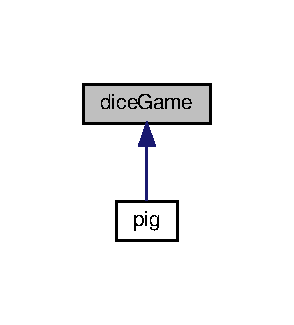
\includegraphics[width=141pt]{classdiceGame__inherit__graph}
\end{center}
\end{figure}


Collaboration diagram for dice\+Game\+:\nopagebreak
\begin{figure}[H]
\begin{center}
\leavevmode
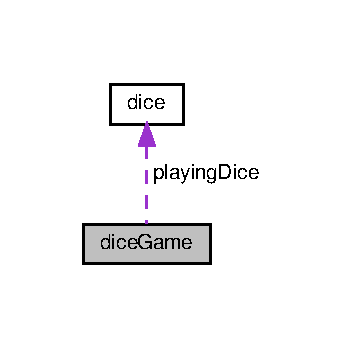
\includegraphics[width=166pt]{classdiceGame__coll__graph}
\end{center}
\end{figure}
\subsection*{Public Member Functions}
\begin{DoxyCompactItemize}
\item 
\hyperlink{classdiceGame_ae964394c63494b6ceb6403e7a66aa4b2}{dice\+Game} ()
\begin{DoxyCompactList}\small\item\em Constructor for creating a dice game. \end{DoxyCompactList}\item 
\hyperlink{classdiceGame_a33c18d6e62bb7599befc405ecbb21402}{$\sim$dice\+Game} ()
\begin{DoxyCompactList}\small\item\em Deconstructor for the dice game which frees memory. \end{DoxyCompactList}\item 
virtual void \hyperlink{classdiceGame_a0620d98347df4779fa620b3b3e239d4e}{play} ()=0
\begin{DoxyCompactList}\small\item\em play function which allows the players to play the game \end{DoxyCompactList}\end{DoxyCompactItemize}
\subsection*{Private Attributes}
\begin{DoxyCompactItemize}
\item 
\mbox{\Hypertarget{classdiceGame_a3a3719c16a28497eba3a36edc73119ad}\label{classdiceGame_a3a3719c16a28497eba3a36edc73119ad}} 
\hyperlink{classdice}{dice} $\ast$ {\bfseries playing\+Dice}
\item 
\mbox{\Hypertarget{classdiceGame_ae67da3cda73d2b5a90bb0ed9365c2b8b}\label{classdiceGame_ae67da3cda73d2b5a90bb0ed9365c2b8b}} 
std\+::vector$<$ \hyperlink{classPlayer}{Player} $\ast$ $>$ {\bfseries player\+List}
\end{DoxyCompactItemize}


\subsection{Detailed Description}
Interface for all dice games to use. 

\begin{DoxyAuthor}{Author}
Owen Hunsburger 250919957
\end{DoxyAuthor}
Provides each dice game with dice and players required 

\subsection{Constructor \& Destructor Documentation}
\mbox{\Hypertarget{classdiceGame_ae964394c63494b6ceb6403e7a66aa4b2}\label{classdiceGame_ae964394c63494b6ceb6403e7a66aa4b2}} 
\index{dice\+Game@{dice\+Game}!dice\+Game@{dice\+Game}}
\index{dice\+Game@{dice\+Game}!dice\+Game@{dice\+Game}}
\subsubsection{\texorpdfstring{dice\+Game()}{diceGame()}}
{\footnotesize\ttfamily dice\+Game\+::dice\+Game (\begin{DoxyParamCaption}{ }\end{DoxyParamCaption})}



Constructor for creating a dice game. 

\begin{DoxyAuthor}{Author}
Owen Hunsburger 250919957 
\end{DoxyAuthor}
\begin{DoxyReturn}{Returns}
a dice game
\end{DoxyReturn}
Creates a new instance of a dice game \mbox{\Hypertarget{classdiceGame_a33c18d6e62bb7599befc405ecbb21402}\label{classdiceGame_a33c18d6e62bb7599befc405ecbb21402}} 
\index{dice\+Game@{dice\+Game}!````~dice\+Game@{$\sim$dice\+Game}}
\index{````~dice\+Game@{$\sim$dice\+Game}!dice\+Game@{dice\+Game}}
\subsubsection{\texorpdfstring{$\sim$dice\+Game()}{~diceGame()}}
{\footnotesize\ttfamily dice\+Game\+::$\sim$dice\+Game (\begin{DoxyParamCaption}{ }\end{DoxyParamCaption})}



Deconstructor for the dice game which frees memory. 

\begin{DoxyAuthor}{Author}
Owen Hunsburger 250919957
\end{DoxyAuthor}
Deletes the dice used in previously made dice game 

\subsection{Member Function Documentation}
\mbox{\Hypertarget{classdiceGame_a0620d98347df4779fa620b3b3e239d4e}\label{classdiceGame_a0620d98347df4779fa620b3b3e239d4e}} 
\index{dice\+Game@{dice\+Game}!play@{play}}
\index{play@{play}!dice\+Game@{dice\+Game}}
\subsubsection{\texorpdfstring{play()}{play()}}
{\footnotesize\ttfamily virtual void dice\+Game\+::play (\begin{DoxyParamCaption}{ }\end{DoxyParamCaption})\hspace{0.3cm}{\ttfamily [pure virtual]}}



play function which allows the players to play the game 

\begin{DoxyAuthor}{Author}
Owen Hunsburger 250919957
\end{DoxyAuthor}
calls the game which implements the game logic and takes user input 

Implemented in \hyperlink{classpig_a83fd8571e2f33ec33f6fafd7efa96571}{pig}.



The documentation for this class was generated from the following files\+:\begin{DoxyCompactItemize}
\item 
Base\+Dice/dice\+Game.\+h\item 
Base\+Dice/dice\+Game.\+cpp\end{DoxyCompactItemize}

\hypertarget{classLeaderBoard}{}\section{Leader\+Board Class Reference}
\label{classLeaderBoard}\index{Leader\+Board@{Leader\+Board}}


Provides Class representation of the \hyperlink{classLeaderBoard}{Leader\+Board} and ways to view the \hyperlink{classLeaderBoard}{Leader\+Board}.  




{\ttfamily \#include $<$Leader\+Board.\+h$>$}

\subsection*{Public Member Functions}
\begin{DoxyCompactItemize}
\item 
\hyperlink{classLeaderBoard_adc7b14c64cca2cddc9cb951f1d5779db}{Leader\+Board} ()
\begin{DoxyCompactList}\small\item\em Constructor for the \hyperlink{classLeaderBoard}{Leader\+Board} gets all the highscore data from the Data file. \end{DoxyCompactList}\item 
void \hyperlink{classLeaderBoard_ae5abb64b73518c25bc32809b5547a87c}{view\+\_\+player} (std\+::string name)
\begin{DoxyCompactList}\small\item\em Method to view the highscores of an individual player. \end{DoxyCompactList}\item 
void \hyperlink{classLeaderBoard_abaa849f35f01657971f8962e9f754ef6}{view\+\_\+highscores} ()
\begin{DoxyCompactList}\small\item\em Method to view the entire \hyperlink{classLeaderBoard}{Leader\+Board} table, Highscores of all players. \end{DoxyCompactList}\end{DoxyCompactItemize}
\subsection*{Private Attributes}
\begin{DoxyCompactItemize}
\item 
\mbox{\Hypertarget{classLeaderBoard_a558a066c4e7b5b2cfe36f14eacc95e62}\label{classLeaderBoard_a558a066c4e7b5b2cfe36f14eacc95e62}} 
std\+::vector$<$ std\+::string $>$ {\bfseries highscores}
\end{DoxyCompactItemize}


\subsection{Detailed Description}
Provides Class representation of the \hyperlink{classLeaderBoard}{Leader\+Board} and ways to view the \hyperlink{classLeaderBoard}{Leader\+Board}. 

Allows any \hyperlink{classPlayer}{Player} while in the menu to view the entire \hyperlink{classLeaderBoard}{Leader\+Board} or the highscores of a specific \hyperlink{classPlayer}{Player} \begin{DoxyAuthor}{Author}
Mark Jaskiewicz 250925120 
\end{DoxyAuthor}


\subsection{Constructor \& Destructor Documentation}
\mbox{\Hypertarget{classLeaderBoard_adc7b14c64cca2cddc9cb951f1d5779db}\label{classLeaderBoard_adc7b14c64cca2cddc9cb951f1d5779db}} 
\index{Leader\+Board@{Leader\+Board}!Leader\+Board@{Leader\+Board}}
\index{Leader\+Board@{Leader\+Board}!Leader\+Board@{Leader\+Board}}
\subsubsection{\texorpdfstring{Leader\+Board()}{LeaderBoard()}}
{\footnotesize\ttfamily Leader\+Board\+::\+Leader\+Board (\begin{DoxyParamCaption}{ }\end{DoxyParamCaption})}



Constructor for the \hyperlink{classLeaderBoard}{Leader\+Board} gets all the highscore data from the Data file. 

\begin{DoxyReturn}{Returns}
returns a vector contains all \hyperlink{classPlayer}{Player} names and highscores, Also every Game name
\end{DoxyReturn}
Uses the Data file defined in The \hyperlink{Player_8h_source}{Player.\+h} file, Skips all unneeded Information Ie. Login info 

\subsection{Member Function Documentation}
\mbox{\Hypertarget{classLeaderBoard_abaa849f35f01657971f8962e9f754ef6}\label{classLeaderBoard_abaa849f35f01657971f8962e9f754ef6}} 
\index{Leader\+Board@{Leader\+Board}!view\+\_\+highscores@{view\+\_\+highscores}}
\index{view\+\_\+highscores@{view\+\_\+highscores}!Leader\+Board@{Leader\+Board}}
\subsubsection{\texorpdfstring{view\+\_\+highscores()}{view\_highscores()}}
{\footnotesize\ttfamily void Leader\+Board\+::view\+\_\+highscores (\begin{DoxyParamCaption}{ }\end{DoxyParamCaption})}



Method to view the entire \hyperlink{classLeaderBoard}{Leader\+Board} table, Highscores of all players. 


\begin{DoxyParams}{Parameters}
{\em None} & \\
\hline
\end{DoxyParams}
\begin{DoxyReturn}{Returns}
void\+: but outputs all players and their respected highscore for each game
\end{DoxyReturn}
Uses the vector created constured to output required info \mbox{\Hypertarget{classLeaderBoard_ae5abb64b73518c25bc32809b5547a87c}\label{classLeaderBoard_ae5abb64b73518c25bc32809b5547a87c}} 
\index{Leader\+Board@{Leader\+Board}!view\+\_\+player@{view\+\_\+player}}
\index{view\+\_\+player@{view\+\_\+player}!Leader\+Board@{Leader\+Board}}
\subsubsection{\texorpdfstring{view\+\_\+player()}{view\_player()}}
{\footnotesize\ttfamily void Leader\+Board\+::view\+\_\+player (\begin{DoxyParamCaption}\item[{std\+::string}]{name }\end{DoxyParamCaption})}



Method to view the highscores of an individual player. 


\begin{DoxyParams}{Parameters}
{\em name,Used} & to specify the players Highscores you wish to view \\
\hline
\end{DoxyParams}
\begin{DoxyReturn}{Returns}
void\+: but outputs to std out the Game names along with the player name and all their highscores
\end{DoxyReturn}
Uses the vector created in constructor to get all required info 

The documentation for this class was generated from the following files\+:\begin{DoxyCompactItemize}
\item 
Leader\+Board/Leader\+Board.\+h\item 
Leader\+Board/Leader\+Board.\+cpp\end{DoxyCompactItemize}

\hypertarget{classMenu}{}\section{Menu Class Reference}
\label{classMenu}\index{Menu@{Menu}}


\hyperlink{classMenu}{Menu} Class represents the text based main menu which allows navigation of our program.  




{\ttfamily \#include $<$Menu.\+h$>$}



Collaboration diagram for Menu\+:\nopagebreak
\begin{figure}[H]
\begin{center}
\leavevmode
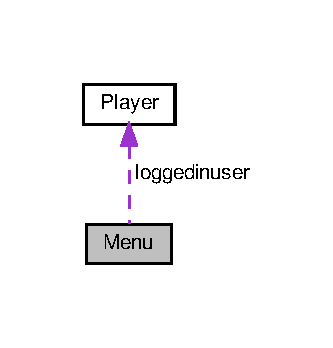
\includegraphics[width=160pt]{classMenu__coll__graph}
\end{center}
\end{figure}
\subsection*{Public Member Functions}
\begin{DoxyCompactItemize}
\item 
\hyperlink{classMenu_ad466dd83355124a6ed958430450bfe94}{Menu} ()
\begin{DoxyCompactList}\small\item\em \hyperlink{classMenu}{Menu} constructor which acts as the main for our program running everything through this. \end{DoxyCompactList}\item 
void \hyperlink{classMenu_ab9be630400e32b048b2f48ebcbc6303e}{register\+User} (std\+::string uname, std\+::string pword)
\begin{DoxyCompactList}\small\item\em Registers the user into the userdata.\+txt database. \end{DoxyCompactList}\item 
void \hyperlink{classMenu_af8c8f162dc3243212f2da97caac85e46}{view\+Leaderboard} ()
\begin{DoxyCompactList}\small\item\em allows user to view the leaderboard section. \end{DoxyCompactList}\item 
\hyperlink{classPlayer}{Player} $\ast$ \hyperlink{classMenu_a5b7acd7315b89b7db11e0791ef6edc44}{login} (std\+::string username, std\+::string password)
\begin{DoxyCompactList}\small\item\em Allows user that is already registered to login. \end{DoxyCompactList}\item 
\hyperlink{classPlayer}{Player} $\ast$ \hyperlink{classMenu_a8a89cf8a328d06d20edf1a807865c8f6}{get\+Logged\+In\+User} ()
\begin{DoxyCompactList}\small\item\em Returns a pointer to the currently logged in user. \end{DoxyCompactList}\item 
std\+::vector$<$ \hyperlink{classPlayer}{Player} $\ast$ $>$ \hyperlink{classMenu_a1a6c905c9a2bcb5bed082baeb2d4929a}{get\+User\+List} ()
\begin{DoxyCompactList}\small\item\em returns the userlist of players currently playing/loggedin. \end{DoxyCompactList}\end{DoxyCompactItemize}
\subsection*{Private Attributes}
\begin{DoxyCompactItemize}
\item 
\mbox{\Hypertarget{classMenu_acf5fcd8a7996710086267c856991b053}\label{classMenu_acf5fcd8a7996710086267c856991b053}} 
std\+::vector$<$ \hyperlink{classPlayer}{Player} $\ast$ $>$ {\bfseries player\+List}
\item 
\mbox{\Hypertarget{classMenu_a9fec21a0fe02ffaf00ff13261a986eb1}\label{classMenu_a9fec21a0fe02ffaf00ff13261a986eb1}} 
\hyperlink{classPlayer}{Player} $\ast$ {\bfseries loggedinuser}
\end{DoxyCompactItemize}


\subsection{Detailed Description}
\hyperlink{classMenu}{Menu} Class represents the text based main menu which allows navigation of our program. 

\hyperlink{classMenu}{Menu} class provides options off the bat to either login, register, check the leaderboard or exit If register is chosen it adds this user to our userdata.\+txt ascii database, Login references the userdata and checks if the uname and pword are valid. leaderboard allows for the display of the entire leaderboard or an individuals highscores. Exit command will exit our program whenever the option is available. The menu allows for navigation and implementation and all our other features. \begin{DoxyAuthor}{Author}
Matthew Costa 250921778 
\end{DoxyAuthor}


\subsection{Constructor \& Destructor Documentation}
\mbox{\Hypertarget{classMenu_ad466dd83355124a6ed958430450bfe94}\label{classMenu_ad466dd83355124a6ed958430450bfe94}} 
\index{Menu@{Menu}!Menu@{Menu}}
\index{Menu@{Menu}!Menu@{Menu}}
\subsubsection{\texorpdfstring{Menu()}{Menu()}}
{\footnotesize\ttfamily Menu\+::\+Menu (\begin{DoxyParamCaption}{ }\end{DoxyParamCaption})}



\hyperlink{classMenu}{Menu} constructor which acts as the main for our program running everything through this. 

\begin{DoxyReturn}{Returns}
n/a  n/a
\end{DoxyReturn}
\hyperlink{classMenu}{Menu} constructor that continues to run until the user enters Exit, It continuously loops to different sections depending on input to allow for the experience of a text based menu. Has multiple verification checks on input and acts as a text based menu for our entire program. 

\subsection{Member Function Documentation}
\mbox{\Hypertarget{classMenu_a8a89cf8a328d06d20edf1a807865c8f6}\label{classMenu_a8a89cf8a328d06d20edf1a807865c8f6}} 
\index{Menu@{Menu}!get\+Logged\+In\+User@{get\+Logged\+In\+User}}
\index{get\+Logged\+In\+User@{get\+Logged\+In\+User}!Menu@{Menu}}
\subsubsection{\texorpdfstring{get\+Logged\+In\+User()}{getLoggedInUser()}}
{\footnotesize\ttfamily \hyperlink{classPlayer}{Player} $\ast$ Menu\+::get\+Logged\+In\+User (\begin{DoxyParamCaption}{ }\end{DoxyParamCaption})}



Returns a pointer to the currently logged in user. 

\begin{DoxyReturn}{Returns}
Pointer to logged in player  n/a
\end{DoxyReturn}
Returns the user that is saved as the logged in user. It returns the player as a player pointer that is stored when a user logs in using the login function. \mbox{\Hypertarget{classMenu_a1a6c905c9a2bcb5bed082baeb2d4929a}\label{classMenu_a1a6c905c9a2bcb5bed082baeb2d4929a}} 
\index{Menu@{Menu}!get\+User\+List@{get\+User\+List}}
\index{get\+User\+List@{get\+User\+List}!Menu@{Menu}}
\subsubsection{\texorpdfstring{get\+User\+List()}{getUserList()}}
{\footnotesize\ttfamily vector$<$ \hyperlink{classPlayer}{Player} $\ast$ $>$ Menu\+::get\+User\+List (\begin{DoxyParamCaption}{ }\end{DoxyParamCaption})}



returns the userlist of players currently playing/loggedin. 

\begin{DoxyReturn}{Returns}
vector of player pointers  n/a
\end{DoxyReturn}
Returns a vector which contains all the players currently logged in or playing the game. This could contain pseudo profiles if a guest is playing the game instead of two logged in players. \mbox{\Hypertarget{classMenu_a5b7acd7315b89b7db11e0791ef6edc44}\label{classMenu_a5b7acd7315b89b7db11e0791ef6edc44}} 
\index{Menu@{Menu}!login@{login}}
\index{login@{login}!Menu@{Menu}}
\subsubsection{\texorpdfstring{login()}{login()}}
{\footnotesize\ttfamily \hyperlink{classPlayer}{Player} $\ast$ Menu\+::login (\begin{DoxyParamCaption}\item[{std\+::string}]{username,  }\item[{std\+::string}]{password }\end{DoxyParamCaption})}



Allows user that is already registered to login. 

\begin{DoxyReturn}{Returns}
Pointer to the player that is logged in  the username and password of the user that is trying to login
\end{DoxyReturn}
Uses the paramaters given to check if the user is able to login. If valid username and password the user is logged in and added to the playerlist. Otherwise it informs the user of invalid credentials. Makes use of the player class to verify by calling ispseudo to see if the player returned was a valid user or a pseudo profile returned. If valid stores this player as the loggedinuser \mbox{\Hypertarget{classMenu_ab9be630400e32b048b2f48ebcbc6303e}\label{classMenu_ab9be630400e32b048b2f48ebcbc6303e}} 
\index{Menu@{Menu}!register\+User@{register\+User}}
\index{register\+User@{register\+User}!Menu@{Menu}}
\subsubsection{\texorpdfstring{register\+User()}{registerUser()}}
{\footnotesize\ttfamily void Menu\+::register\+User (\begin{DoxyParamCaption}\item[{std\+::string}]{uname,  }\item[{std\+::string}]{pword }\end{DoxyParamCaption})}



Registers the user into the userdata.\+txt database. 

\begin{DoxyReturn}{Returns}
void  the username and password of the user that is trying to register
\end{DoxyReturn}
Uses the paramaters given to register the user by adding them to the userdata.\+txt file. Method checks for an existing profile with these credentials and if it finds one informs the user of a failed register. Method also checks if the params include a comma and informs the user that the registry cant happen with commas. \mbox{\Hypertarget{classMenu_af8c8f162dc3243212f2da97caac85e46}\label{classMenu_af8c8f162dc3243212f2da97caac85e46}} 
\index{Menu@{Menu}!view\+Leaderboard@{view\+Leaderboard}}
\index{view\+Leaderboard@{view\+Leaderboard}!Menu@{Menu}}
\subsubsection{\texorpdfstring{view\+Leaderboard()}{viewLeaderboard()}}
{\footnotesize\ttfamily void Menu\+::view\+Leaderboard (\begin{DoxyParamCaption}{ }\end{DoxyParamCaption})}



allows user to view the leaderboard section. 

\begin{DoxyReturn}{Returns}
void  n/a
\end{DoxyReturn}
Allows user to view the leaderboard with one of two options. Either the user can choose to view one players leaderboard values or the entire leaderboard. Depending on the choice two different methods from the leaderboard class are called. 

The documentation for this class was generated from the following files\+:\begin{DoxyCompactItemize}
\item 
Base\+Menu/Menu.\+h\item 
Base\+Menu/Menu.\+cpp\end{DoxyCompactItemize}

\hypertarget{classpig}{}\section{pig Class Reference}
\label{classpig}\index{pig@{pig}}


Contains all the logic required for pig, a dice game.  




{\ttfamily \#include $<$pig.\+h$>$}



Inheritance diagram for pig\+:\nopagebreak
\begin{figure}[H]
\begin{center}
\leavevmode
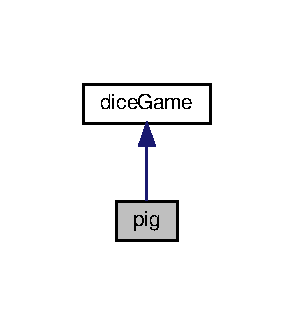
\includegraphics[width=141pt]{classpig__inherit__graph}
\end{center}
\end{figure}


Collaboration diagram for pig\+:\nopagebreak
\begin{figure}[H]
\begin{center}
\leavevmode
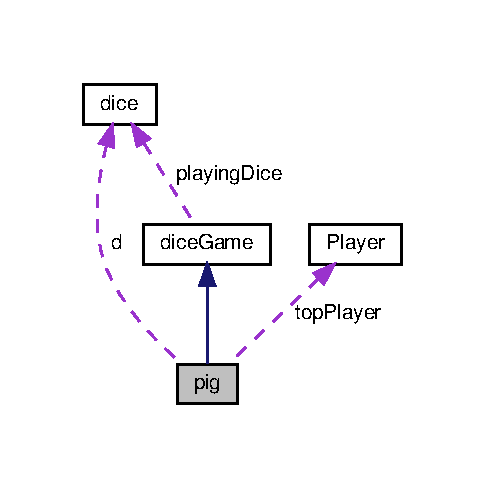
\includegraphics[width=233pt]{classpig__coll__graph}
\end{center}
\end{figure}
\subsection*{Public Member Functions}
\begin{DoxyCompactItemize}
\item 
\mbox{\Hypertarget{classpig_a14f66c6f931e7f88e887d1af8e06eadc}\label{classpig_a14f66c6f931e7f88e887d1af8e06eadc}} 
{\bfseries pig} (std\+::vector$<$ \hyperlink{classPlayer}{Player} $\ast$$>$ players)
\item 
void \hyperlink{classpig_a83fd8571e2f33ec33f6fafd7efa96571}{play} ()
\begin{DoxyCompactList}\small\item\em play function which allows the players to play the game \end{DoxyCompactList}\end{DoxyCompactItemize}
\subsection*{Private Attributes}
\begin{DoxyCompactItemize}
\item 
\mbox{\Hypertarget{classpig_a548163e47b2f1b82fd9fb6c20caf7092}\label{classpig_a548163e47b2f1b82fd9fb6c20caf7092}} 
std\+::vector$<$ \hyperlink{classPlayer}{Player} $\ast$ $>$ {\bfseries player\+List}
\item 
\mbox{\Hypertarget{classpig_ae4fe8f68279a723773d0041f4210c315}\label{classpig_ae4fe8f68279a723773d0041f4210c315}} 
int {\bfseries num\+Of\+Players}
\item 
\mbox{\Hypertarget{classpig_ad7c324c675cf9b720c3144be43093d83}\label{classpig_ad7c324c675cf9b720c3144be43093d83}} 
\hyperlink{classdice}{dice} $\ast$ {\bfseries d}
\item 
\mbox{\Hypertarget{classpig_a7ef22bd927c220866f15abcb28f33f32}\label{classpig_a7ef22bd927c220866f15abcb28f33f32}} 
int {\bfseries score}
\item 
\mbox{\Hypertarget{classpig_aa79cb61f2628fe37edd36ad76af4d081}\label{classpig_aa79cb61f2628fe37edd36ad76af4d081}} 
int {\bfseries current\+Roll}
\item 
\mbox{\Hypertarget{classpig_abfb581424e14beb6250acf5df111a417}\label{classpig_abfb581424e14beb6250acf5df111a417}} 
bool {\bfseries playing}
\item 
\mbox{\Hypertarget{classpig_a6a6c1566b19486cceb33910c902348b0}\label{classpig_a6a6c1566b19486cceb33910c902348b0}} 
std\+::string {\bfseries input}
\item 
\mbox{\Hypertarget{classpig_ac35d859274db9267f8b7039b50e65bfe}\label{classpig_ac35d859274db9267f8b7039b50e65bfe}} 
std\+::string {\bfseries plyr}
\item 
\mbox{\Hypertarget{classpig_a5159b3cb3879e33b9bf1adad4c2c270b}\label{classpig_a5159b3cb3879e33b9bf1adad4c2c270b}} 
int {\bfseries top\+Score}
\item 
\mbox{\Hypertarget{classpig_a98a7c1492538a8c643a42eba071ca7e4}\label{classpig_a98a7c1492538a8c643a42eba071ca7e4}} 
\hyperlink{classPlayer}{Player} {\bfseries top\+Player}
\item 
\mbox{\Hypertarget{classpig_a1d5787bef5d4a72458e84c4b094b00fe}\label{classpig_a1d5787bef5d4a72458e84c4b094b00fe}} 
bool {\bfseries tie}
\item 
\mbox{\Hypertarget{classpig_a99faed0cf1d6a816db10e100531f698f}\label{classpig_a99faed0cf1d6a816db10e100531f698f}} 
int {\bfseries count}
\end{DoxyCompactItemize}


\subsection{Detailed Description}
Contains all the logic required for pig, a dice game. 

\begin{DoxyAuthor}{Author}
Owen Hunsburger 250919957
\end{DoxyAuthor}
Uses dice object and a vector of players, uses \hyperlink{classdiceGame}{dice\+Game} as a template 

\subsection{Member Function Documentation}
\mbox{\Hypertarget{classpig_a83fd8571e2f33ec33f6fafd7efa96571}\label{classpig_a83fd8571e2f33ec33f6fafd7efa96571}} 
\index{pig@{pig}!play@{play}}
\index{play@{play}!pig@{pig}}
\subsubsection{\texorpdfstring{play()}{play()}}
{\footnotesize\ttfamily void pig\+::play (\begin{DoxyParamCaption}{ }\end{DoxyParamCaption})\hspace{0.3cm}{\ttfamily [virtual]}}



play function which allows the players to play the game 

\begin{DoxyAuthor}{Author}
Owen Hunsburger 250919957
\end{DoxyAuthor}
calls the game which implements the game logic and takes user input 

Implements \hyperlink{classdiceGame_a0620d98347df4779fa620b3b3e239d4e}{dice\+Game}.



The documentation for this class was generated from the following files\+:\begin{DoxyCompactItemize}
\item 
Pig/pig.\+h\item 
Pig/pig.\+cpp\end{DoxyCompactItemize}

\hypertarget{classPlayer}{}\section{Player Class Reference}
\label{classPlayer}\index{Player@{Player}}


Provides a class representation of everything a player has in and associated with a game.  




{\ttfamily \#include $<$Player.\+h$>$}

\subsection*{Public Member Functions}
\begin{DoxyCompactItemize}
\item 
\hyperlink{classPlayer_affe0cc3cb714f6deb4e62f0c0d3f1fd8}{Player} ()
\begin{DoxyCompactList}\small\item\em Empty constructor which makes a temporary profile with default values for variables. \end{DoxyCompactList}\item 
\hyperlink{classPlayer_a61d2a5c3a5f6a6e4a408ba802337af51}{Player} (std\+::string uname, std\+::string pword)
\begin{DoxyCompactList}\small\item\em Constructor which Checks records for a user and logs them in. \end{DoxyCompactList}\item 
std\+::string \hyperlink{classPlayer_a73c00480e9459d52998262f23f6fc5dc}{get\+Username} ()
\begin{DoxyCompactList}\small\item\em Getter method for the \hyperlink{classPlayer}{Player}\textquotesingle{}s username. \end{DoxyCompactList}\item 
void \hyperlink{classPlayer_a8fc488bcda5714ae92466d2936380787}{set\+Username} (std\+::string uname)
\begin{DoxyCompactList}\small\item\em Setter method for the \hyperlink{classPlayer}{Player}\textquotesingle{}s username. \end{DoxyCompactList}\item 
std\+::string \hyperlink{classPlayer_aef0e6355f59ecc9a72dfda313c603b5e}{get\+Password} ()
\begin{DoxyCompactList}\small\item\em Getter method for the \hyperlink{classPlayer}{Player}\textquotesingle{}s password. \end{DoxyCompactList}\item 
void \hyperlink{classPlayer_afff83ec36cc74b248cf1a723ab0c2b6a}{set\+Password} (std\+::string pword)
\begin{DoxyCompactList}\small\item\em Setter method for the \hyperlink{classPlayer}{Player}\textquotesingle{}s password. \end{DoxyCompactList}\item 
double \hyperlink{classPlayer_a0e9f70886f4a7544422931103e59ea26}{get\+Balance} ()
\begin{DoxyCompactList}\small\item\em Getter method for the \hyperlink{classPlayer}{Player}\textquotesingle{}s balance. \end{DoxyCompactList}\item 
void \hyperlink{classPlayer_a7bdcb72d5d22f6f7c1dfa48d960b6d73}{set\+Balance} (double bal)
\begin{DoxyCompactList}\small\item\em Setter method for the \hyperlink{classPlayer}{Player}\textquotesingle{}s balance. \end{DoxyCompactList}\item 
double \hyperlink{classPlayer_a42286b7c54da75f7b64200796f149d4c}{get\+Highscore} (std\+::string game)
\begin{DoxyCompactList}\small\item\em Getter method for the \hyperlink{classPlayer}{Player}\textquotesingle{}s highscore. \end{DoxyCompactList}\item 
void \hyperlink{classPlayer_ae77a5ec07cea02f94c7c8bc9830e2521}{set\+Highscore} (std\+::string game, double score)
\begin{DoxyCompactList}\small\item\em Setter method for the \hyperlink{classPlayer}{Player}\textquotesingle{}s highscore for the given game. \end{DoxyCompactList}\item 
double \hyperlink{classPlayer_a0aade73735727e68e4f07734e76c875a}{get\+Current\+Game\+Score} ()
\begin{DoxyCompactList}\small\item\em Getter method for the \hyperlink{classPlayer}{Player}\textquotesingle{}s current game score. \end{DoxyCompactList}\item 
void \hyperlink{classPlayer_a1b2af56d4beb6e7a7961b3b572b42bdb}{set\+Current\+Game\+Score} (double score)
\begin{DoxyCompactList}\small\item\em Setter method for the \hyperlink{classPlayer}{Player}\textquotesingle{}s current game score. \end{DoxyCompactList}\item 
bool \hyperlink{classPlayer_a50aa73eae22ec3435d3de2e556bd1fec}{is\+Pseudo} ()
\begin{DoxyCompactList}\small\item\em Checks if the user object is a temp or is a pseudo profile. \end{DoxyCompactList}\item 
std\+::vector$<$ \hyperlink{classcard}{card} $\ast$ $>$ \hyperlink{classPlayer_a5117d4863ff28cd0bf522cfe34995c27}{get\+Current\+Hand} ()
\begin{DoxyCompactList}\small\item\em Getter method for the \hyperlink{classPlayer}{Player}\textquotesingle{}s current hand in the game they are playing. \end{DoxyCompactList}\item 
void \hyperlink{classPlayer_a8a4e0a62953bad66dd6dd18f28619ead}{set\+Current\+Hand} (std\+::vector$<$ \hyperlink{classcard}{card} $\ast$$>$ hand)
\begin{DoxyCompactList}\small\item\em Setter method for the \hyperlink{classPlayer}{Player}\textquotesingle{}s current hand. \end{DoxyCompactList}\end{DoxyCompactItemize}
\subsection*{Private Attributes}
\begin{DoxyCompactItemize}
\item 
\mbox{\Hypertarget{classPlayer_af6823e27c17ba6ed5d2b4713abbe4d5a}\label{classPlayer_af6823e27c17ba6ed5d2b4713abbe4d5a}} 
std\+::string {\bfseries username}
\item 
\mbox{\Hypertarget{classPlayer_a62136f186be055500d69c835d8593f39}\label{classPlayer_a62136f186be055500d69c835d8593f39}} 
std\+::string {\bfseries password}
\item 
\mbox{\Hypertarget{classPlayer_a13f91e1079f0a76f2e8fb8aaa421b9b6}\label{classPlayer_a13f91e1079f0a76f2e8fb8aaa421b9b6}} 
double {\bfseries balance}
\item 
\mbox{\Hypertarget{classPlayer_a8737097eeb7a21cfe36e6a873ca0db28}\label{classPlayer_a8737097eeb7a21cfe36e6a873ca0db28}} 
bool {\bfseries pseudo}
\item 
\mbox{\Hypertarget{classPlayer_ae520913dfc9e2939dcc23bb3a3a97741}\label{classPlayer_ae520913dfc9e2939dcc23bb3a3a97741}} 
std\+::vector$<$ \hyperlink{classcard}{card} $\ast$ $>$ {\bfseries current\+Hand}
\item 
\mbox{\Hypertarget{classPlayer_a6d6dacc63c26bba93641fabc50997259}\label{classPlayer_a6d6dacc63c26bba93641fabc50997259}} 
double {\bfseries current\+Game\+Score}
\end{DoxyCompactItemize}


\subsection{Detailed Description}
Provides a class representation of everything a player has in and associated with a game. 

\begin{DoxyAuthor}{Author}
Thomas Morphew 250921958 The \hyperlink{classPlayer}{Player} class represents someone playing the game. All Players will have a username, password, and a balance that they can bring between gambling games. An instance of this class has quick access data stored in its instance variables. Changing these values will also write them to a file for recording purposes. A \hyperlink{classPlayer}{Player} in a card game may have a \char`\"{}hand\char`\"{} of cards to keep track of what cards are available. Players can be both \char`\"{}real\char`\"{} or \char`\"{}pseudo\char`\"{} (which effectively means temporary). This duality of the class lets it represent AI\textquotesingle{}s that games may need to run or double as a temporary profile for a trial player. 
\end{DoxyAuthor}


\subsection{Constructor \& Destructor Documentation}
\mbox{\Hypertarget{classPlayer_affe0cc3cb714f6deb4e62f0c0d3f1fd8}\label{classPlayer_affe0cc3cb714f6deb4e62f0c0d3f1fd8}} 
\index{Player@{Player}!Player@{Player}}
\index{Player@{Player}!Player@{Player}}
\subsubsection{\texorpdfstring{Player()}{Player()}\hspace{0.1cm}{\footnotesize\ttfamily [1/2]}}
{\footnotesize\ttfamily Player\+::\+Player (\begin{DoxyParamCaption}{ }\end{DoxyParamCaption})}



Empty constructor which makes a temporary profile with default values for variables. 

\begin{DoxyReturn}{Returns}
a pseudo profile with default values for instance variables.
\end{DoxyReturn}
An empty constructor which makes a temporary profile with default values for variables. This can be used as a temporary player, ideal for AI in games. \mbox{\Hypertarget{classPlayer_a61d2a5c3a5f6a6e4a408ba802337af51}\label{classPlayer_a61d2a5c3a5f6a6e4a408ba802337af51}} 
\index{Player@{Player}!Player@{Player}}
\index{Player@{Player}!Player@{Player}}
\subsubsection{\texorpdfstring{Player()}{Player()}\hspace{0.1cm}{\footnotesize\ttfamily [2/2]}}
{\footnotesize\ttfamily Player\+::\+Player (\begin{DoxyParamCaption}\item[{std\+::string}]{uname,  }\item[{std\+::string}]{pword }\end{DoxyParamCaption})}



Constructor which Checks records for a user and logs them in. 


\begin{DoxyParams}{Parameters}
{\em uname} & is the username of a player\textquotesingle{}s record \\
\hline
{\em pword} & is the password of a player\textquotesingle{}s record \\
\hline
\end{DoxyParams}
\begin{DoxyReturn}{Returns}
a player\textquotesingle{}s profile with their saved data loaded into the object if login successful, otherwise it returns a temporary profile.
\end{DoxyReturn}
Primary constructor for \hyperlink{classPlayer}{Player} class, it performs a login with the associated memory file and then fills the class\textquotesingle{}s instance variables with the correct values from the file. If the login is unsuccessful, then a pseudo profile is returned instead. 

\subsection{Member Function Documentation}
\mbox{\Hypertarget{classPlayer_a0e9f70886f4a7544422931103e59ea26}\label{classPlayer_a0e9f70886f4a7544422931103e59ea26}} 
\index{Player@{Player}!get\+Balance@{get\+Balance}}
\index{get\+Balance@{get\+Balance}!Player@{Player}}
\subsubsection{\texorpdfstring{get\+Balance()}{getBalance()}}
{\footnotesize\ttfamily double Player\+::get\+Balance (\begin{DoxyParamCaption}{ }\end{DoxyParamCaption})}



Getter method for the \hyperlink{classPlayer}{Player}\textquotesingle{}s balance. 

\begin{DoxyReturn}{Returns}
the balance for the \hyperlink{classPlayer}{Player} object
\end{DoxyReturn}
Getter method for the \hyperlink{classPlayer}{Player}\textquotesingle{}s balance. Useful for keeping track of money between games. \mbox{\Hypertarget{classPlayer_a0aade73735727e68e4f07734e76c875a}\label{classPlayer_a0aade73735727e68e4f07734e76c875a}} 
\index{Player@{Player}!get\+Current\+Game\+Score@{get\+Current\+Game\+Score}}
\index{get\+Current\+Game\+Score@{get\+Current\+Game\+Score}!Player@{Player}}
\subsubsection{\texorpdfstring{get\+Current\+Game\+Score()}{getCurrentGameScore()}}
{\footnotesize\ttfamily double Player\+::get\+Current\+Game\+Score (\begin{DoxyParamCaption}{ }\end{DoxyParamCaption})}



Getter method for the \hyperlink{classPlayer}{Player}\textquotesingle{}s current game score. 

\begin{DoxyReturn}{Returns}
the current score for the \hyperlink{classPlayer}{Player} in the game they are playing
\end{DoxyReturn}
Gets the current score of the \hyperlink{classPlayer}{Player} for the game they are currently playing in. \mbox{\Hypertarget{classPlayer_a5117d4863ff28cd0bf522cfe34995c27}\label{classPlayer_a5117d4863ff28cd0bf522cfe34995c27}} 
\index{Player@{Player}!get\+Current\+Hand@{get\+Current\+Hand}}
\index{get\+Current\+Hand@{get\+Current\+Hand}!Player@{Player}}
\subsubsection{\texorpdfstring{get\+Current\+Hand()}{getCurrentHand()}}
{\footnotesize\ttfamily std\+::vector$<$ \hyperlink{classcard}{card} $\ast$ $>$ Player\+::get\+Current\+Hand (\begin{DoxyParamCaption}{ }\end{DoxyParamCaption})}



Getter method for the \hyperlink{classPlayer}{Player}\textquotesingle{}s current hand in the game they are playing. 

\begin{DoxyReturn}{Returns}
the current hand of cards for the \hyperlink{classPlayer}{Player} in the game they are playing
\end{DoxyReturn}
Gets the current hand of cards the \hyperlink{classPlayer}{Player} has for the game they are currently playing in. \mbox{\Hypertarget{classPlayer_a42286b7c54da75f7b64200796f149d4c}\label{classPlayer_a42286b7c54da75f7b64200796f149d4c}} 
\index{Player@{Player}!get\+Highscore@{get\+Highscore}}
\index{get\+Highscore@{get\+Highscore}!Player@{Player}}
\subsubsection{\texorpdfstring{get\+Highscore()}{getHighscore()}}
{\footnotesize\ttfamily double Player\+::get\+Highscore (\begin{DoxyParamCaption}\item[{std\+::string}]{game }\end{DoxyParamCaption})}



Getter method for the \hyperlink{classPlayer}{Player}\textquotesingle{}s highscore. 


\begin{DoxyParams}{Parameters}
{\em game} & is the name of the game in the record file \\
\hline
\end{DoxyParams}
\begin{DoxyReturn}{Returns}
the highscore for the \hyperlink{classPlayer}{Player} for the game given by the parameter
\end{DoxyReturn}
Gets the highscore of the \hyperlink{classPlayer}{Player} for the game given by the parameter. Accesses the record file directly, may perform slowly for large files. \mbox{\Hypertarget{classPlayer_aef0e6355f59ecc9a72dfda313c603b5e}\label{classPlayer_aef0e6355f59ecc9a72dfda313c603b5e}} 
\index{Player@{Player}!get\+Password@{get\+Password}}
\index{get\+Password@{get\+Password}!Player@{Player}}
\subsubsection{\texorpdfstring{get\+Password()}{getPassword()}}
{\footnotesize\ttfamily std\+::string Player\+::get\+Password (\begin{DoxyParamCaption}{ }\end{DoxyParamCaption})}



Getter method for the \hyperlink{classPlayer}{Player}\textquotesingle{}s password. 

\begin{DoxyReturn}{Returns}
the password for the \hyperlink{classPlayer}{Player} object
\end{DoxyReturn}
Getter method for the \hyperlink{classPlayer}{Player}\textquotesingle{}s password. Useful for logging in (security). \mbox{\Hypertarget{classPlayer_a73c00480e9459d52998262f23f6fc5dc}\label{classPlayer_a73c00480e9459d52998262f23f6fc5dc}} 
\index{Player@{Player}!get\+Username@{get\+Username}}
\index{get\+Username@{get\+Username}!Player@{Player}}
\subsubsection{\texorpdfstring{get\+Username()}{getUsername()}}
{\footnotesize\ttfamily std\+::string Player\+::get\+Username (\begin{DoxyParamCaption}{ }\end{DoxyParamCaption})}



Getter method for the \hyperlink{classPlayer}{Player}\textquotesingle{}s username. 

\begin{DoxyReturn}{Returns}
the username for the \hyperlink{classPlayer}{Player} object
\end{DoxyReturn}
Getter method for the \hyperlink{classPlayer}{Player}\textquotesingle{}s username. Useful for displaying in games. \mbox{\Hypertarget{classPlayer_a50aa73eae22ec3435d3de2e556bd1fec}\label{classPlayer_a50aa73eae22ec3435d3de2e556bd1fec}} 
\index{Player@{Player}!is\+Pseudo@{is\+Pseudo}}
\index{is\+Pseudo@{is\+Pseudo}!Player@{Player}}
\subsubsection{\texorpdfstring{is\+Pseudo()}{isPseudo()}}
{\footnotesize\ttfamily bool Player\+::is\+Pseudo (\begin{DoxyParamCaption}{ }\end{DoxyParamCaption})}



Checks if the user object is a temp or is a pseudo profile. 

\begin{DoxyReturn}{Returns}
a bool, true if the \hyperlink{classPlayer}{Player} is a pseudo profile or false otherwise.
\end{DoxyReturn}
Checks if the player is a pseudo (temporary) player. Pseudo players are temporary and do not save to the record file. \mbox{\Hypertarget{classPlayer_a7bdcb72d5d22f6f7c1dfa48d960b6d73}\label{classPlayer_a7bdcb72d5d22f6f7c1dfa48d960b6d73}} 
\index{Player@{Player}!set\+Balance@{set\+Balance}}
\index{set\+Balance@{set\+Balance}!Player@{Player}}
\subsubsection{\texorpdfstring{set\+Balance()}{setBalance()}}
{\footnotesize\ttfamily void Player\+::set\+Balance (\begin{DoxyParamCaption}\item[{double}]{bal }\end{DoxyParamCaption})}



Setter method for the \hyperlink{classPlayer}{Player}\textquotesingle{}s balance. 


\begin{DoxyParams}{Parameters}
{\em bal} & is the new balance for the record \\
\hline
\end{DoxyParams}
\begin{DoxyReturn}{Returns}
void
\end{DoxyReturn}
Sets the balance for the object and also saves it to the record file. \mbox{\Hypertarget{classPlayer_a1b2af56d4beb6e7a7961b3b572b42bdb}\label{classPlayer_a1b2af56d4beb6e7a7961b3b572b42bdb}} 
\index{Player@{Player}!set\+Current\+Game\+Score@{set\+Current\+Game\+Score}}
\index{set\+Current\+Game\+Score@{set\+Current\+Game\+Score}!Player@{Player}}
\subsubsection{\texorpdfstring{set\+Current\+Game\+Score()}{setCurrentGameScore()}}
{\footnotesize\ttfamily void Player\+::set\+Current\+Game\+Score (\begin{DoxyParamCaption}\item[{double}]{score }\end{DoxyParamCaption})}



Setter method for the \hyperlink{classPlayer}{Player}\textquotesingle{}s current game score. 


\begin{DoxyParams}{Parameters}
{\em score} & is the new score of the current game to save to the record file \\
\hline
\end{DoxyParams}
\begin{DoxyReturn}{Returns}
void
\end{DoxyReturn}
Sets the current score of the \hyperlink{classPlayer}{Player} for the game they are current playing in. \mbox{\Hypertarget{classPlayer_a8a4e0a62953bad66dd6dd18f28619ead}\label{classPlayer_a8a4e0a62953bad66dd6dd18f28619ead}} 
\index{Player@{Player}!set\+Current\+Hand@{set\+Current\+Hand}}
\index{set\+Current\+Hand@{set\+Current\+Hand}!Player@{Player}}
\subsubsection{\texorpdfstring{set\+Current\+Hand()}{setCurrentHand()}}
{\footnotesize\ttfamily void Player\+::set\+Current\+Hand (\begin{DoxyParamCaption}\item[{std\+::vector$<$ \hyperlink{classcard}{card} $\ast$$>$}]{hand }\end{DoxyParamCaption})}



Setter method for the \hyperlink{classPlayer}{Player}\textquotesingle{}s current hand. 


\begin{DoxyParams}{Parameters}
{\em hand} & is the new hand of the current game the player is in. \\
\hline
\end{DoxyParams}
\begin{DoxyReturn}{Returns}
void
\end{DoxyReturn}
Sets the current hand of cards the \hyperlink{classPlayer}{Player} has for the game they are current playing in. \mbox{\Hypertarget{classPlayer_ae77a5ec07cea02f94c7c8bc9830e2521}\label{classPlayer_ae77a5ec07cea02f94c7c8bc9830e2521}} 
\index{Player@{Player}!set\+Highscore@{set\+Highscore}}
\index{set\+Highscore@{set\+Highscore}!Player@{Player}}
\subsubsection{\texorpdfstring{set\+Highscore()}{setHighscore()}}
{\footnotesize\ttfamily void Player\+::set\+Highscore (\begin{DoxyParamCaption}\item[{std\+::string}]{game,  }\item[{double}]{score }\end{DoxyParamCaption})}



Setter method for the \hyperlink{classPlayer}{Player}\textquotesingle{}s highscore for the given game. 


\begin{DoxyParams}{Parameters}
{\em game} & is the name of the game in the record file \\
\hline
{\em score} & is the new score of the game to save to the record file \\
\hline
\end{DoxyParams}
\begin{DoxyReturn}{Returns}
void
\end{DoxyReturn}
Sets the highscore of the \hyperlink{classPlayer}{Player} for the game given by the parameter. Saves the new highscore to record file. \mbox{\Hypertarget{classPlayer_afff83ec36cc74b248cf1a723ab0c2b6a}\label{classPlayer_afff83ec36cc74b248cf1a723ab0c2b6a}} 
\index{Player@{Player}!set\+Password@{set\+Password}}
\index{set\+Password@{set\+Password}!Player@{Player}}
\subsubsection{\texorpdfstring{set\+Password()}{setPassword()}}
{\footnotesize\ttfamily void Player\+::set\+Password (\begin{DoxyParamCaption}\item[{std\+::string}]{pword }\end{DoxyParamCaption})}



Setter method for the \hyperlink{classPlayer}{Player}\textquotesingle{}s password. 


\begin{DoxyParams}{Parameters}
{\em pword} & is the new password for the record \\
\hline
\end{DoxyParams}
\begin{DoxyReturn}{Returns}
void
\end{DoxyReturn}
Sets the password for the object and also saves it to the record file. \mbox{\Hypertarget{classPlayer_a8fc488bcda5714ae92466d2936380787}\label{classPlayer_a8fc488bcda5714ae92466d2936380787}} 
\index{Player@{Player}!set\+Username@{set\+Username}}
\index{set\+Username@{set\+Username}!Player@{Player}}
\subsubsection{\texorpdfstring{set\+Username()}{setUsername()}}
{\footnotesize\ttfamily void Player\+::set\+Username (\begin{DoxyParamCaption}\item[{std\+::string}]{uname }\end{DoxyParamCaption})}



Setter method for the \hyperlink{classPlayer}{Player}\textquotesingle{}s username. 


\begin{DoxyParams}{Parameters}
{\em uname} & is the new username for the record \\
\hline
\end{DoxyParams}
\begin{DoxyReturn}{Returns}
void
\end{DoxyReturn}
Sets the username for the object and also saves it to the record file if it is not in use. 

The documentation for this class was generated from the following files\+:\begin{DoxyCompactItemize}
\item 
Base\+Player/Player.\+h\item 
Base\+Player/Player.\+cpp\end{DoxyCompactItemize}

\hypertarget{classWar}{}\section{War Class Reference}
\label{classWar}\index{War@{War}}


\hyperlink{classWar}{War} class contains all game logic for the card game war.  




{\ttfamily \#include $<$War.\+h$>$}



Inheritance diagram for War\+:\nopagebreak
\begin{figure}[H]
\begin{center}
\leavevmode
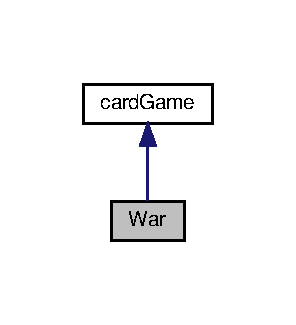
\includegraphics[width=142pt]{classWar__inherit__graph}
\end{center}
\end{figure}


Collaboration diagram for War\+:\nopagebreak
\begin{figure}[H]
\begin{center}
\leavevmode
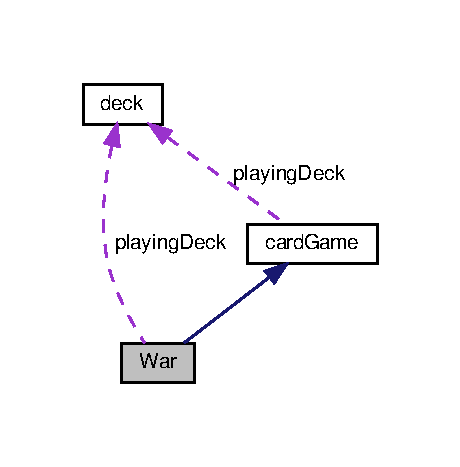
\includegraphics[width=221pt]{classWar__coll__graph}
\end{center}
\end{figure}
\subsection*{Public Member Functions}
\begin{DoxyCompactItemize}
\item 
\mbox{\Hypertarget{classWar_a354b86ad426e3e5323d3d642e5bedc99}\label{classWar_a354b86ad426e3e5323d3d642e5bedc99}} 
{\bfseries War} (std\+::vector$<$ \hyperlink{classPlayer}{Player} $\ast$$>$ players)
\item 
void \hyperlink{classWar_a507414bb7608a837b7b884827795de81}{play} ()
\begin{DoxyCompactList}\small\item\em play function contains all game logic, run to play \end{DoxyCompactList}\end{DoxyCompactItemize}
\subsection*{Private Attributes}
\begin{DoxyCompactItemize}
\item 
\mbox{\Hypertarget{classWar_aba0ff3d35af3cb6fdfcc30ca98e84c6e}\label{classWar_aba0ff3d35af3cb6fdfcc30ca98e84c6e}} 
\hyperlink{classdeck}{deck} $\ast$ {\bfseries playing\+Deck}
\item 
\mbox{\Hypertarget{classWar_add456d46ce43425c60b21b06c1e6706a}\label{classWar_add456d46ce43425c60b21b06c1e6706a}} 
std\+::vector$<$ \hyperlink{classPlayer}{Player} $\ast$ $>$ {\bfseries player\+List}
\end{DoxyCompactItemize}


\subsection{Detailed Description}
\hyperlink{classWar}{War} class contains all game logic for the card game war. 

\hyperlink{classWar}{War} class contains all game logic for the card game war, uses base card game class as a template \begin{DoxyAuthor}{Author}
Jacob Ross 250892852 
\end{DoxyAuthor}


\subsection{Member Function Documentation}
\mbox{\Hypertarget{classWar_a507414bb7608a837b7b884827795de81}\label{classWar_a507414bb7608a837b7b884827795de81}} 
\index{War@{War}!play@{play}}
\index{play@{play}!War@{War}}
\subsubsection{\texorpdfstring{play()}{play()}}
{\footnotesize\ttfamily void War\+::play (\begin{DoxyParamCaption}{ }\end{DoxyParamCaption})\hspace{0.3cm}{\ttfamily [virtual]}}



play function contains all game logic, run to play 

play function contains all game logic, implentation of this function is completely up to game designer \begin{DoxyAuthor}{Author}
Jacob Ross 250892852 
\end{DoxyAuthor}


Implements \hyperlink{classcardGame_ae8e04249f37f61e3adfa03cfbad3b021}{card\+Game}.



The documentation for this class was generated from the following files\+:\begin{DoxyCompactItemize}
\item 
War/War.\+h\item 
War/War.\+cpp\end{DoxyCompactItemize}

%--- End generated contents ---

% Index
\backmatter
\newpage
\phantomsection
\clearemptydoublepage
\addcontentsline{toc}{chapter}{Index}
\printindex

\end{document}
